\documentclass[../ProgettoTecWeb2.tex]{subfiles}

\begin{document}
\section{Risultati di una ricerca}
	La pagina con i risultati di una ricerca che abbia prodotto risultati è molto simile alle pagine delle news, recensioni, etc. e ne presenta pregi e difetti. Da notare che anche in questo caso viene utilizzata una visualizzazione a griglia (sarebbe da preferire invece una visualizzazione a lista soprattutto in questo caaso). In alto troviamo riportato ciò che abbiamo cercato con la possibilità di applicare il filtro per effettuare la ricerca solamente tra le news, tra le recensioni, tra le anteprime oppure tra i contenuti speciali.
	\begin{figure} [H]
		\centering
		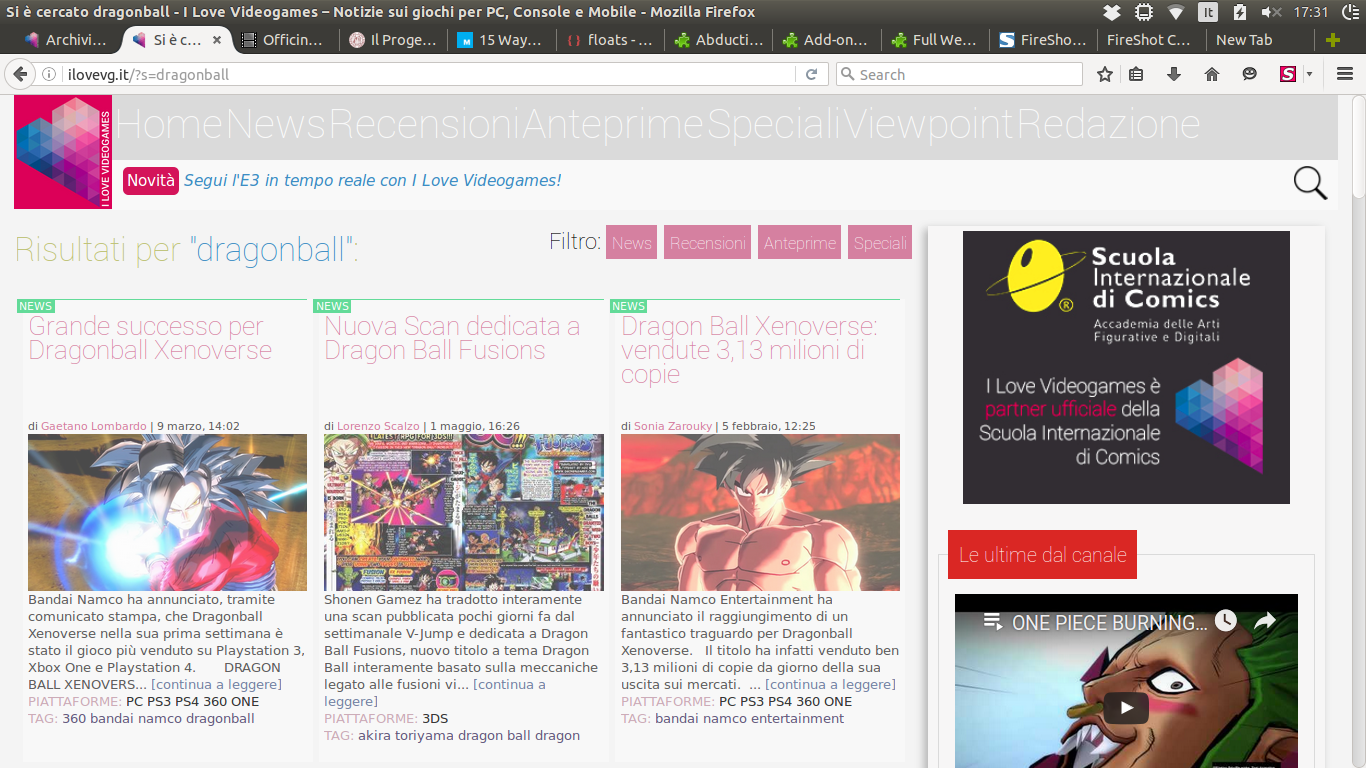
\includegraphics[scale=0.2]{img/RicercaConRisultati}
		\caption{Pagina dei risultati cercando ``dragonball''}
	\end{figure}

	Nel caso in cui la ricerca non produca alcun risultato invece viene visualizzata una pagina che spiega appunto che ciò che è stato cercato non è associato ad alcun contenuto del sito.
	\begin{figure} [H]
		\centering
		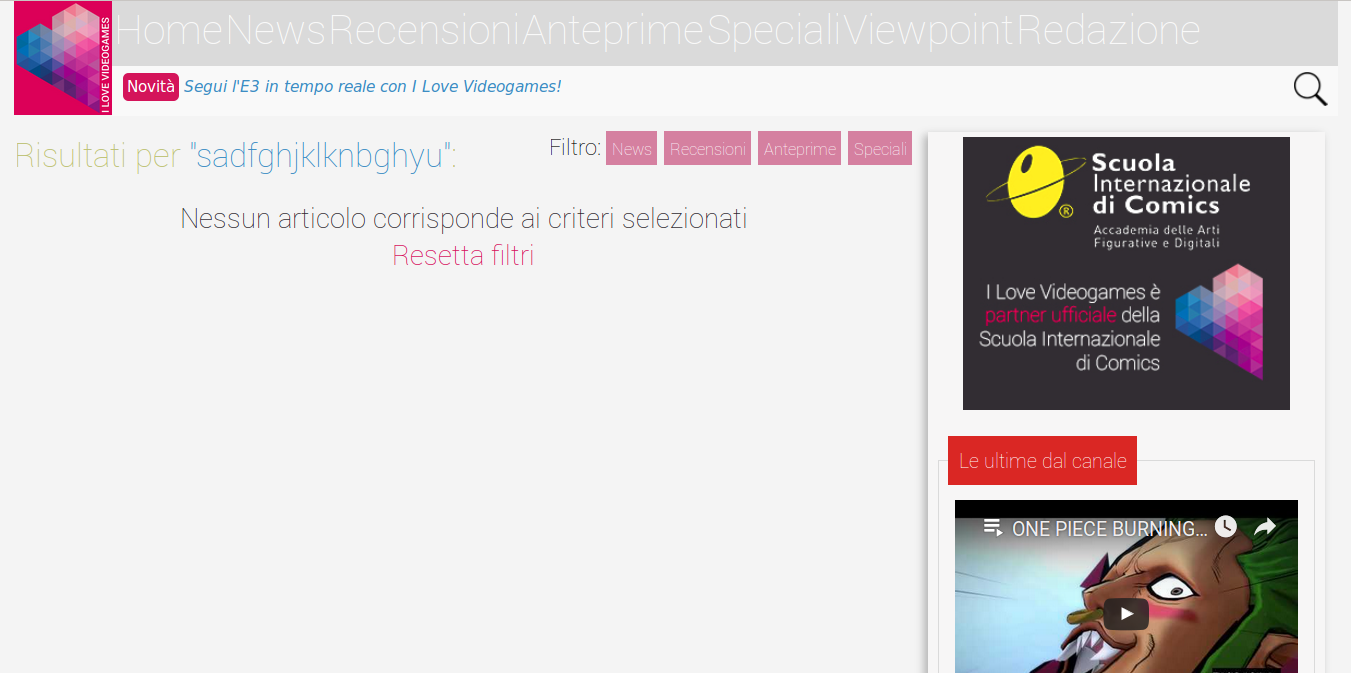
\includegraphics[scale=0.2]{img/RicercaNoRisultati}
		\caption{Pagina dei risultati cercando ``sadfghjklknbghyu''}
	\end{figure}

\end{document}